\documentclass[twoside]{book}

% Packages required by doxygen
\usepackage{fixltx2e}
\usepackage{calc}
\usepackage{doxygen}
\usepackage[export]{adjustbox} % also loads graphicx
\usepackage{graphicx}
\usepackage[utf8]{inputenc}
\usepackage{makeidx}
\usepackage{multicol}
\usepackage{multirow}
\PassOptionsToPackage{warn}{textcomp}
\usepackage{textcomp}
\usepackage[nointegrals]{wasysym}
\usepackage[table]{xcolor}

% Font selection
\usepackage[T1]{fontenc}
\usepackage[scaled=.90]{helvet}
\usepackage{courier}
\usepackage{amssymb}
\usepackage{sectsty}
\renewcommand{\familydefault}{\sfdefault}
\allsectionsfont{%
  \fontseries{bc}\selectfont%
  \color{darkgray}%
}
\renewcommand{\DoxyLabelFont}{%
  \fontseries{bc}\selectfont%
  \color{darkgray}%
}
\newcommand{\+}{\discretionary{\mbox{\scriptsize$\hookleftarrow$}}{}{}}

% Page & text layout
\usepackage{geometry}
\geometry{%
  a4paper,%
  top=2.5cm,%
  bottom=2.5cm,%
  left=2.5cm,%
  right=2.5cm%
}
\tolerance=750
\hfuzz=15pt
\hbadness=750
\setlength{\emergencystretch}{15pt}
\setlength{\parindent}{0cm}
\setlength{\parskip}{3ex plus 2ex minus 2ex}
\makeatletter
\renewcommand{\paragraph}{%
  \@startsection{paragraph}{4}{0ex}{-1.0ex}{1.0ex}{%
    \normalfont\normalsize\bfseries\SS@parafont%
  }%
}
\renewcommand{\subparagraph}{%
  \@startsection{subparagraph}{5}{0ex}{-1.0ex}{1.0ex}{%
    \normalfont\normalsize\bfseries\SS@subparafont%
  }%
}
\makeatother

% Headers & footers
\usepackage{fancyhdr}
\pagestyle{fancyplain}
\fancyhead[LE]{\fancyplain{}{\bfseries\thepage}}
\fancyhead[CE]{\fancyplain{}{}}
\fancyhead[RE]{\fancyplain{}{\bfseries\leftmark}}
\fancyhead[LO]{\fancyplain{}{\bfseries\rightmark}}
\fancyhead[CO]{\fancyplain{}{}}
\fancyhead[RO]{\fancyplain{}{\bfseries\thepage}}
\fancyfoot[LE]{\fancyplain{}{}}
\fancyfoot[CE]{\fancyplain{}{}}
\fancyfoot[RE]{\fancyplain{}{\bfseries\scriptsize Generated by Doxygen }}
\fancyfoot[LO]{\fancyplain{}{\bfseries\scriptsize Generated by Doxygen }}
\fancyfoot[CO]{\fancyplain{}{}}
\fancyfoot[RO]{\fancyplain{}{}}
\renewcommand{\footrulewidth}{0.4pt}
\renewcommand{\chaptermark}[1]{%
  \markboth{#1}{}%
}
\renewcommand{\sectionmark}[1]{%
  \markright{\thesection\ #1}%
}

% Indices & bibliography
\usepackage{natbib}
\usepackage[titles]{tocloft}
\setcounter{tocdepth}{3}
\setcounter{secnumdepth}{5}
\makeindex

% Hyperlinks (required, but should be loaded last)
\usepackage{ifpdf}
\ifpdf
  \usepackage[pdftex,pagebackref=true]{hyperref}
\else
  \usepackage[ps2pdf,pagebackref=true]{hyperref}
\fi
\hypersetup{%
  colorlinks=true,%
  linkcolor=blue,%
  citecolor=blue,%
  unicode%
}

% Custom commands
\newcommand{\clearemptydoublepage}{%
  \newpage{\pagestyle{empty}\cleardoublepage}%
}

\usepackage{caption}
\captionsetup{labelsep=space,justification=centering,font={bf},singlelinecheck=off,skip=4pt,position=top}

%===== C O N T E N T S =====

\begin{document}

% Titlepage & ToC
\hypersetup{pageanchor=false,
             bookmarksnumbered=true,
             pdfencoding=unicode
            }
\pagenumbering{alph}
\begin{titlepage}
\vspace*{7cm}
\begin{center}%
{\Large Tracer }\\
\vspace*{1cm}
{\large Generated by Doxygen 1.8.13}\\
\end{center}
\end{titlepage}
\clearemptydoublepage
\pagenumbering{roman}
\tableofcontents
\clearemptydoublepage
\pagenumbering{arabic}
\hypersetup{pageanchor=true}

%--- Begin generated contents ---
\chapter{Hierarchical Index}
\section{Class Hierarchy}
This inheritance list is sorted roughly, but not completely, alphabetically\+:\begin{DoxyCompactList}
\item \contentsline{section}{camera}{\pageref{classcamera}}{}
\item \contentsline{section}{hit\+\_\+record}{\pageref{structhit__record}}{}
\item \contentsline{section}{hittable}{\pageref{classhittable}}{}
\begin{DoxyCompactList}
\item \contentsline{section}{hittable\+\_\+list}{\pageref{classhittable__list}}{}
\item \contentsline{section}{sphere}{\pageref{classsphere}}{}
\end{DoxyCompactList}
\item \contentsline{section}{material}{\pageref{classmaterial}}{}
\begin{DoxyCompactList}
\item \contentsline{section}{dielectric}{\pageref{classdielectric}}{}
\item \contentsline{section}{lambertian}{\pageref{classlambertian}}{}
\item \contentsline{section}{lambertian}{\pageref{classlambertian}}{}
\item \contentsline{section}{metal}{\pageref{classmetal}}{}
\item \contentsline{section}{metal}{\pageref{classmetal}}{}
\end{DoxyCompactList}
\item \contentsline{section}{ray}{\pageref{classray}}{}
\item \contentsline{section}{vec3}{\pageref{classvec3}}{}
\end{DoxyCompactList}

\chapter{Class Index}
\section{Class List}
Here are the classes, structs, unions and interfaces with brief descriptions\+:\begin{DoxyCompactList}
\item\contentsline{section}{\hyperlink{classcamera}{camera} }{\pageref{classcamera}}{}
\item\contentsline{section}{\hyperlink{classdielectric}{dielectric} }{\pageref{classdielectric}}{}
\item\contentsline{section}{\hyperlink{structhit__record}{hit\+\_\+record} }{\pageref{structhit__record}}{}
\item\contentsline{section}{\hyperlink{classhittable}{hittable} }{\pageref{classhittable}}{}
\item\contentsline{section}{\hyperlink{classhittable__list}{hittable\+\_\+list} }{\pageref{classhittable__list}}{}
\item\contentsline{section}{\hyperlink{classlambertian}{lambertian} }{\pageref{classlambertian}}{}
\item\contentsline{section}{\hyperlink{classmaterial}{material} }{\pageref{classmaterial}}{}
\item\contentsline{section}{\hyperlink{classmetal}{metal} }{\pageref{classmetal}}{}
\item\contentsline{section}{\hyperlink{classray}{ray} }{\pageref{classray}}{}
\item\contentsline{section}{\hyperlink{classsphere}{sphere} }{\pageref{classsphere}}{}
\item\contentsline{section}{\hyperlink{classvec3}{vec3} }{\pageref{classvec3}}{}
\end{DoxyCompactList}

\chapter{Class Documentation}
\hypertarget{classcamera}{}\section{camera Class Reference}
\label{classcamera}\index{camera@{camera}}


Collaboration diagram for camera\+:
\nopagebreak
\begin{figure}[H]
\begin{center}
\leavevmode
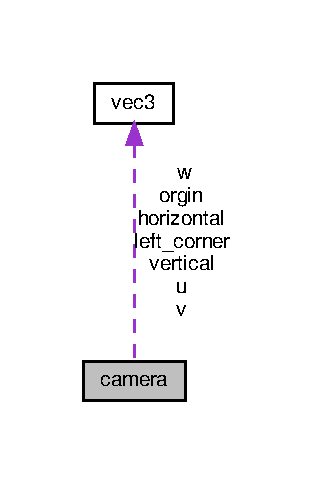
\includegraphics[width=151pt]{classcamera__coll__graph}
\end{center}
\end{figure}
\subsection*{Public Member Functions}
\begin{DoxyCompactItemize}
\item 
\mbox{\Hypertarget{classcamera_acdf970a12643e5ea1c594ff7623942f4}\label{classcamera_acdf970a12643e5ea1c594ff7623942f4}} 
{\bfseries camera} (\hyperlink{classvec3}{vec3} from, \hyperlink{classvec3}{vec3} lookat, \hyperlink{classvec3}{vec3} vup, float deg, float aspect, float aperture, float focus)
\item 
\mbox{\Hypertarget{classcamera_a8c47e02062b903e907cb0dad2de62211}\label{classcamera_a8c47e02062b903e907cb0dad2de62211}} 
\hyperlink{classray}{ray} {\bfseries view} (float a, float b)
\end{DoxyCompactItemize}
\subsection*{Public Attributes}
\begin{DoxyCompactItemize}
\item 
\mbox{\Hypertarget{classcamera_a69e10fd2cc480c82ab94764bdab76a10}\label{classcamera_a69e10fd2cc480c82ab94764bdab76a10}} 
float {\bfseries width}
\item 
\mbox{\Hypertarget{classcamera_a5b8898243a5c86b93420ebf7acf8e38e}\label{classcamera_a5b8898243a5c86b93420ebf7acf8e38e}} 
float {\bfseries height}
\item 
\mbox{\Hypertarget{classcamera_a6972f535b7b21cb967d62b4711bfcd08}\label{classcamera_a6972f535b7b21cb967d62b4711bfcd08}} 
\hyperlink{classvec3}{vec3} {\bfseries orgin}
\item 
\mbox{\Hypertarget{classcamera_a4f33036cda2e0e4a85333ceebbad6344}\label{classcamera_a4f33036cda2e0e4a85333ceebbad6344}} 
\hyperlink{classvec3}{vec3} {\bfseries left\+\_\+corner}
\item 
\mbox{\Hypertarget{classcamera_a195d6ef80d6cd3d4ef6dbdf6333799d3}\label{classcamera_a195d6ef80d6cd3d4ef6dbdf6333799d3}} 
\hyperlink{classvec3}{vec3} {\bfseries horizontal}
\item 
\mbox{\Hypertarget{classcamera_a27c92c40ba0833359e87ecf095cc4d22}\label{classcamera_a27c92c40ba0833359e87ecf095cc4d22}} 
\hyperlink{classvec3}{vec3} {\bfseries vertical}
\item 
\mbox{\Hypertarget{classcamera_a610b4723a2dc8dbeefc815fe99116719}\label{classcamera_a610b4723a2dc8dbeefc815fe99116719}} 
\hyperlink{classvec3}{vec3} {\bfseries u}
\item 
\mbox{\Hypertarget{classcamera_a056e047e57d62a35813f8c5d7bfa78cb}\label{classcamera_a056e047e57d62a35813f8c5d7bfa78cb}} 
\hyperlink{classvec3}{vec3} {\bfseries v}
\item 
\mbox{\Hypertarget{classcamera_a67a4be1092662ed5b399a396ba61df50}\label{classcamera_a67a4be1092662ed5b399a396ba61df50}} 
\hyperlink{classvec3}{vec3} {\bfseries w}
\item 
\mbox{\Hypertarget{classcamera_a4ec3ef650f65d9575cc21c44117b6d4c}\label{classcamera_a4ec3ef650f65d9575cc21c44117b6d4c}} 
float {\bfseries lens\+\_\+radius}
\end{DoxyCompactItemize}


The documentation for this class was generated from the following file\+:\begin{DoxyCompactItemize}
\item 
camera.\+h\end{DoxyCompactItemize}

\hypertarget{classdielectric}{}\section{dielectric Class Reference}
\label{classdielectric}\index{dielectric@{dielectric}}


Inheritance diagram for dielectric\+:
\nopagebreak
\begin{figure}[H]
\begin{center}
\leavevmode
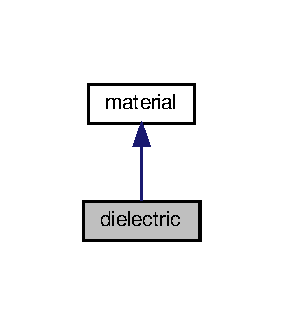
\includegraphics[width=136pt]{classdielectric__inherit__graph}
\end{center}
\end{figure}


Collaboration diagram for dielectric\+:
\nopagebreak
\begin{figure}[H]
\begin{center}
\leavevmode
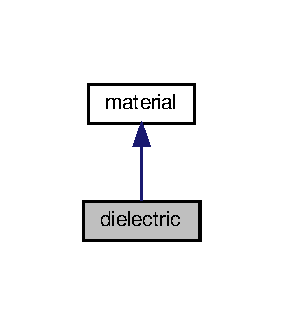
\includegraphics[width=136pt]{classdielectric__coll__graph}
\end{center}
\end{figure}
\subsection*{Public Member Functions}
\begin{DoxyCompactItemize}
\item 
\mbox{\Hypertarget{classdielectric_a85d94cef67b68990254c985c602a6295}\label{classdielectric_a85d94cef67b68990254c985c602a6295}} 
{\bfseries dielectric} (float id)
\item 
\mbox{\Hypertarget{classdielectric_a3fc10ebe6567e530ce72463b45f88a58}\label{classdielectric_a3fc10ebe6567e530ce72463b45f88a58}} 
bool {\bfseries scatter} (const \hyperlink{classray}{ray} \&r\+\_\+in, const \hyperlink{structhit__record}{hit\+\_\+record} \&rec, \hyperlink{classvec3}{vec3} \&att, \hyperlink{classray}{ray} \&scat) const
\end{DoxyCompactItemize}
\subsection*{Public Attributes}
\begin{DoxyCompactItemize}
\item 
\mbox{\Hypertarget{classdielectric_aae76571f5f1161abca541ecfdd86a60c}\label{classdielectric_aae76571f5f1161abca541ecfdd86a60c}} 
float {\bfseries idx}
\end{DoxyCompactItemize}


The documentation for this class was generated from the following file\+:\begin{DoxyCompactItemize}
\item 
hittable.\+h\end{DoxyCompactItemize}

\hypertarget{structhit__record}{}\section{hit\+\_\+record Struct Reference}
\label{structhit__record}\index{hit\+\_\+record@{hit\+\_\+record}}


Collaboration diagram for hit\+\_\+record\+:
\nopagebreak
\begin{figure}[H]
\begin{center}
\leavevmode
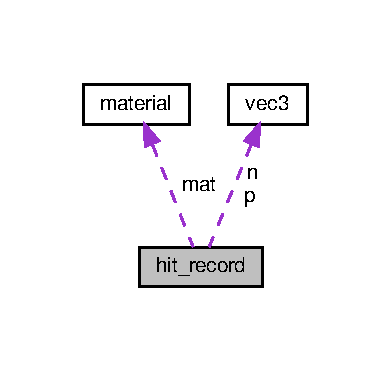
\includegraphics[width=188pt]{structhit__record__coll__graph}
\end{center}
\end{figure}
\subsection*{Public Attributes}
\begin{DoxyCompactItemize}
\item 
\mbox{\Hypertarget{structhit__record_a7f01fe93ab07f09e943f772c8f4d86b4}\label{structhit__record_a7f01fe93ab07f09e943f772c8f4d86b4}} 
float {\bfseries t}
\item 
\mbox{\Hypertarget{structhit__record_af0d915768e7418302348430cb788836b}\label{structhit__record_af0d915768e7418302348430cb788836b}} 
\hyperlink{classvec3}{vec3} {\bfseries p}
\item 
\mbox{\Hypertarget{structhit__record_a3314f2cb9d948b210769d0439c92a02e}\label{structhit__record_a3314f2cb9d948b210769d0439c92a02e}} 
\hyperlink{classvec3}{vec3} {\bfseries n}
\item 
\mbox{\Hypertarget{structhit__record_afa2214a5eefe5e0280deef41ab2ad8d0}\label{structhit__record_afa2214a5eefe5e0280deef41ab2ad8d0}} 
\hyperlink{classmaterial}{material} $\ast$ {\bfseries mat}
\end{DoxyCompactItemize}


The documentation for this struct was generated from the following file\+:\begin{DoxyCompactItemize}
\item 
hittable.\+h\end{DoxyCompactItemize}

\hypertarget{classhittable}{}\section{hittable Class Reference}
\label{classhittable}\index{hittable@{hittable}}


Inheritance diagram for hittable\+:
\nopagebreak
\begin{figure}[H]
\begin{center}
\leavevmode
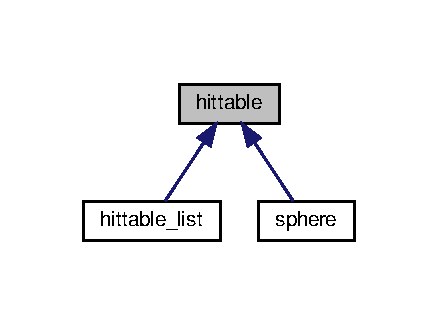
\includegraphics[width=210pt]{classhittable__inherit__graph}
\end{center}
\end{figure}
\subsection*{Public Member Functions}
\begin{DoxyCompactItemize}
\item 
\mbox{\Hypertarget{classhittable_aa1b6671f373a166f9bd44148f2a0fe23}\label{classhittable_aa1b6671f373a166f9bd44148f2a0fe23}} 
virtual bool {\bfseries hit} (const \hyperlink{classray}{ray} \&r, float min, float max, \hyperlink{structhit__record}{hit\+\_\+record} \&rec) const =0
\end{DoxyCompactItemize}


The documentation for this class was generated from the following file\+:\begin{DoxyCompactItemize}
\item 
hittable.\+h\end{DoxyCompactItemize}

\hypertarget{classhittable__list}{}\section{hittable\+\_\+list Class Reference}
\label{classhittable__list}\index{hittable\+\_\+list@{hittable\+\_\+list}}


Inheritance diagram for hittable\+\_\+list\+:
\nopagebreak
\begin{figure}[H]
\begin{center}
\leavevmode
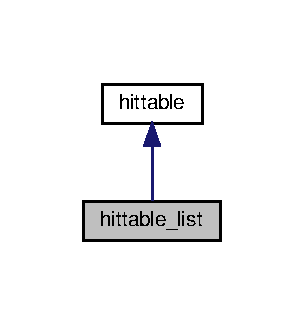
\includegraphics[width=146pt]{classhittable__list__inherit__graph}
\end{center}
\end{figure}


Collaboration diagram for hittable\+\_\+list\+:
\nopagebreak
\begin{figure}[H]
\begin{center}
\leavevmode
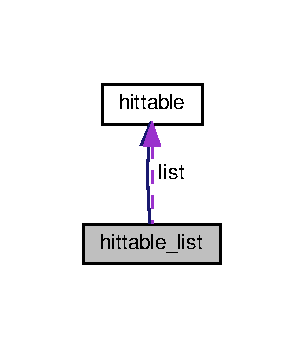
\includegraphics[width=146pt]{classhittable__list__coll__graph}
\end{center}
\end{figure}
\subsection*{Public Member Functions}
\begin{DoxyCompactItemize}
\item 
\mbox{\Hypertarget{classhittable__list_a8f3a3cfa10a2e0b9aa2619d5a5118a61}\label{classhittable__list_a8f3a3cfa10a2e0b9aa2619d5a5118a61}} 
\+\_\+\+\_\+device\+\_\+\+\_\+ {\bfseries hittable\+\_\+list} (\hyperlink{classhittable}{hittable} $\ast$$\ast$a, int b)
\item 
\mbox{\Hypertarget{classhittable__list_a9e03abf8064faef066a3abb312955871}\label{classhittable__list_a9e03abf8064faef066a3abb312955871}} 
\+\_\+\+\_\+device\+\_\+\+\_\+ bool {\bfseries hit} (const \hyperlink{classray}{ray} \&r, float min, float max, \hyperlink{structhit__record}{hit\+\_\+record} \&rec) const
\end{DoxyCompactItemize}
\subsection*{Public Attributes}
\begin{DoxyCompactItemize}
\item 
\mbox{\Hypertarget{classhittable__list_a1f3915d3aa44d03f08ee1a43896573cf}\label{classhittable__list_a1f3915d3aa44d03f08ee1a43896573cf}} 
\hyperlink{classhittable}{hittable} $\ast$$\ast$ {\bfseries list}
\item 
\mbox{\Hypertarget{classhittable__list_aebe3fd61e949b8237dc2dcad01260820}\label{classhittable__list_aebe3fd61e949b8237dc2dcad01260820}} 
int {\bfseries list\+\_\+size}
\end{DoxyCompactItemize}


The documentation for this class was generated from the following file\+:\begin{DoxyCompactItemize}
\item 
hittablelist.\+h\end{DoxyCompactItemize}

\hypertarget{classlambertian}{}\section{lambertian Class Reference}
\label{classlambertian}\index{lambertian@{lambertian}}


Inheritance diagram for lambertian\+:
\nopagebreak
\begin{figure}[H]
\begin{center}
\leavevmode
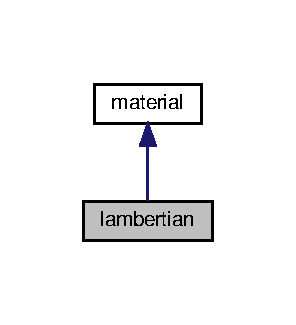
\includegraphics[width=142pt]{classlambertian__inherit__graph}
\end{center}
\end{figure}


Collaboration diagram for lambertian\+:
\nopagebreak
\begin{figure}[H]
\begin{center}
\leavevmode
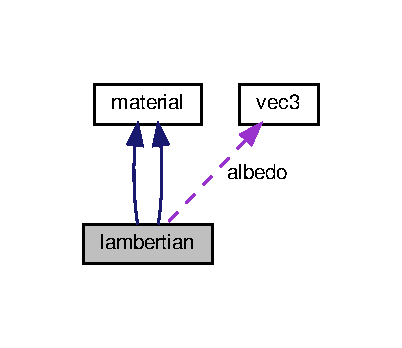
\includegraphics[width=193pt]{classlambertian__coll__graph}
\end{center}
\end{figure}
\subsection*{Public Member Functions}
\begin{DoxyCompactItemize}
\item 
\mbox{\Hypertarget{classlambertian_aaff523a9a978e937a82739909acf316c}\label{classlambertian_aaff523a9a978e937a82739909acf316c}} 
{\bfseries lambertian} (const \hyperlink{classvec3}{vec3} \&a)
\item 
\mbox{\Hypertarget{classlambertian_a191e17273b069e21fc0f4b7fed8337f9}\label{classlambertian_a191e17273b069e21fc0f4b7fed8337f9}} 
bool {\bfseries scatter} (const \hyperlink{classray}{ray} \&r\+\_\+in, const \hyperlink{structhit__record}{hit\+\_\+record} \&rec, \hyperlink{classvec3}{vec3} \&att, \hyperlink{classray}{ray} \&scat) const
\item 
\mbox{\Hypertarget{classlambertian_aaff523a9a978e937a82739909acf316c}\label{classlambertian_aaff523a9a978e937a82739909acf316c}} 
{\bfseries lambertian} (const \hyperlink{classvec3}{vec3} \&a)
\item 
\mbox{\Hypertarget{classlambertian_a7610f6ebbc037003adfb4a8ad7b36871}\label{classlambertian_a7610f6ebbc037003adfb4a8ad7b36871}} 
virtual bool {\bfseries scatter} (const \hyperlink{classray}{ray} \&r\+\_\+in, const \hyperlink{structhit__record}{hit\+\_\+record} \&rec, \hyperlink{classvec3}{vec3} \&att, \hyperlink{classray}{ray} \&scat)
\end{DoxyCompactItemize}
\subsection*{Public Attributes}
\begin{DoxyCompactItemize}
\item 
\mbox{\Hypertarget{classlambertian_a81dc7cd414273c1bec5409e6bfe18f95}\label{classlambertian_a81dc7cd414273c1bec5409e6bfe18f95}} 
\hyperlink{classvec3}{vec3} {\bfseries albedo}
\end{DoxyCompactItemize}


The documentation for this class was generated from the following files\+:\begin{DoxyCompactItemize}
\item 
hittable.\+h\item 
material.\+h\end{DoxyCompactItemize}

\hypertarget{classmaterial}{}\section{material Class Reference}
\label{classmaterial}\index{material@{material}}


Inheritance diagram for material\+:
\nopagebreak
\begin{figure}[H]
\begin{center}
\leavevmode
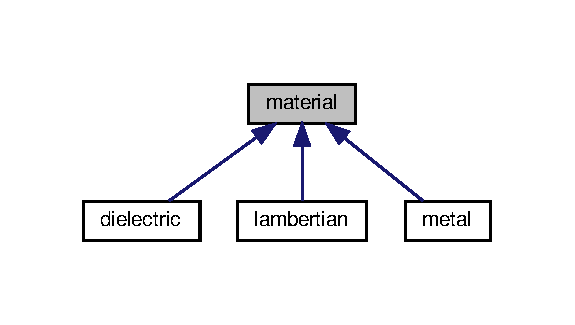
\includegraphics[width=276pt]{classmaterial__inherit__graph}
\end{center}
\end{figure}
\subsection*{Public Member Functions}
\begin{DoxyCompactItemize}
\item 
\mbox{\Hypertarget{classmaterial_a6ffef7f6d9b22511129af150c4142852}\label{classmaterial_a6ffef7f6d9b22511129af150c4142852}} 
virtual bool {\bfseries scatter} (const \hyperlink{classray}{ray} \&r\+\_\+in, const \hyperlink{structhit__record}{hit\+\_\+record} \&rec, \hyperlink{classvec3}{vec3} \&att, \hyperlink{classray}{ray} \&scat) const =0
\item 
\mbox{\Hypertarget{classmaterial_a78cfbe3c64a6adf08dc016ecdb1789a6}\label{classmaterial_a78cfbe3c64a6adf08dc016ecdb1789a6}} 
virtual bool {\bfseries scatter} (const \hyperlink{classray}{ray} \&r\+\_\+in, struct \hyperlink{structhit__record}{hit\+\_\+record} $\ast$rec, \hyperlink{classvec3}{vec3} \&att, \hyperlink{classray}{ray} \&scat) const =0
\end{DoxyCompactItemize}


The documentation for this class was generated from the following files\+:\begin{DoxyCompactItemize}
\item 
hittable.\+h\item 
material.\+h\end{DoxyCompactItemize}

\hypertarget{classmetal}{}\section{metal Class Reference}
\label{classmetal}\index{metal@{metal}}


Inheritance diagram for metal\+:
\nopagebreak
\begin{figure}[H]
\begin{center}
\leavevmode
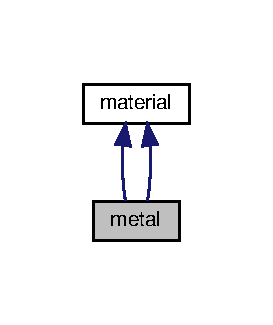
\includegraphics[width=131pt]{classmetal__inherit__graph}
\end{center}
\end{figure}


Collaboration diagram for metal\+:
\nopagebreak
\begin{figure}[H]
\begin{center}
\leavevmode
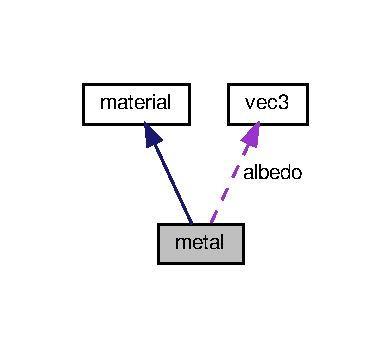
\includegraphics[width=188pt]{classmetal__coll__graph}
\end{center}
\end{figure}
\subsection*{Public Member Functions}
\begin{DoxyCompactItemize}
\item 
\mbox{\Hypertarget{classmetal_a7624f5dc09c2c990ff870eac0aed8ebf}\label{classmetal_a7624f5dc09c2c990ff870eac0aed8ebf}} 
{\bfseries metal} (const \hyperlink{classvec3}{vec3} \&a, float fuz)
\item 
\mbox{\Hypertarget{classmetal_a894ce1be986fbe57fa211bc34cf93384}\label{classmetal_a894ce1be986fbe57fa211bc34cf93384}} 
bool {\bfseries scatter} (const \hyperlink{classray}{ray} \&r\+\_\+in, const \hyperlink{structhit__record}{hit\+\_\+record} \&rec, \hyperlink{classvec3}{vec3} \&att, \hyperlink{classray}{ray} \&scat) const
\item 
\mbox{\Hypertarget{classmetal_afabfe136a55e444d6fe4f85718691b42}\label{classmetal_afabfe136a55e444d6fe4f85718691b42}} 
{\bfseries metal} (const \hyperlink{classvec3}{vec3} \&a)
\item 
\mbox{\Hypertarget{classmetal_ac5fe2b3f2868c5e7a7a118a5efc31be0}\label{classmetal_ac5fe2b3f2868c5e7a7a118a5efc31be0}} 
bool {\bfseries scatter} (const \hyperlink{classray}{ray} \&r\+\_\+in, const \hyperlink{structhit__record}{hit\+\_\+record} \&rec, \hyperlink{classvec3}{vec3} \&att, \hyperlink{classray}{ray} \&scat)
\end{DoxyCompactItemize}
\subsection*{Public Attributes}
\begin{DoxyCompactItemize}
\item 
\mbox{\Hypertarget{classmetal_a7c16624a6f180f58c3bda5558c71e7c1}\label{classmetal_a7c16624a6f180f58c3bda5558c71e7c1}} 
\hyperlink{classvec3}{vec3} {\bfseries albedo}
\item 
\mbox{\Hypertarget{classmetal_a7b1a155f70bf086fc84c4c17d1e6f88c}\label{classmetal_a7b1a155f70bf086fc84c4c17d1e6f88c}} 
float {\bfseries fuzz}
\end{DoxyCompactItemize}


The documentation for this class was generated from the following files\+:\begin{DoxyCompactItemize}
\item 
hittable.\+h\item 
material.\+h\end{DoxyCompactItemize}

\hypertarget{classray}{}\section{ray Class Reference}
\label{classray}\index{ray@{ray}}


Collaboration diagram for ray\+:
\nopagebreak
\begin{figure}[H]
\begin{center}
\leavevmode
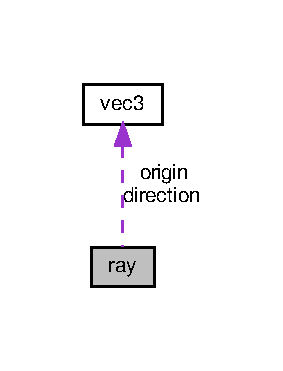
\includegraphics[width=136pt]{classray__coll__graph}
\end{center}
\end{figure}
\subsection*{Public Member Functions}
\begin{DoxyCompactItemize}
\item 
\mbox{\Hypertarget{classray_ac94b9080a724c7bd62600165b41017a4}\label{classray_ac94b9080a724c7bd62600165b41017a4}} 
{\bfseries ray} (const \hyperlink{classvec3}{vec3} \&a, const \hyperlink{classvec3}{vec3} \&b)
\item 
\mbox{\Hypertarget{classray_aa978996b740c24be643e76a7f273d3e0}\label{classray_aa978996b740c24be643e76a7f273d3e0}} 
\hyperlink{classvec3}{vec3} {\bfseries position} (const float \&t) const
\end{DoxyCompactItemize}
\subsection*{Public Attributes}
\begin{DoxyCompactItemize}
\item 
\mbox{\Hypertarget{classray_a355df5fbaf73ad092e7bb95364d8fb81}\label{classray_a355df5fbaf73ad092e7bb95364d8fb81}} 
\hyperlink{classvec3}{vec3} {\bfseries orgin}
\item 
\mbox{\Hypertarget{classray_a60c0e437ff2dbea2eb409b0ba68018c4}\label{classray_a60c0e437ff2dbea2eb409b0ba68018c4}} 
\hyperlink{classvec3}{vec3} {\bfseries direction}
\end{DoxyCompactItemize}


The documentation for this class was generated from the following file\+:\begin{DoxyCompactItemize}
\item 
ray.\+h\end{DoxyCompactItemize}

\hypertarget{classsphere}{}\section{sphere Class Reference}
\label{classsphere}\index{sphere@{sphere}}


Inheritance diagram for sphere\+:
\nopagebreak
\begin{figure}[H]
\begin{center}
\leavevmode
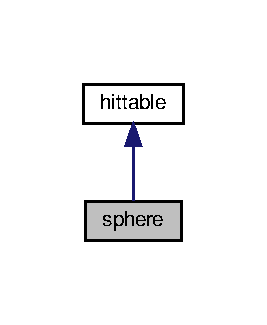
\includegraphics[width=128pt]{classsphere__inherit__graph}
\end{center}
\end{figure}


Collaboration diagram for sphere\+:
\nopagebreak
\begin{figure}[H]
\begin{center}
\leavevmode
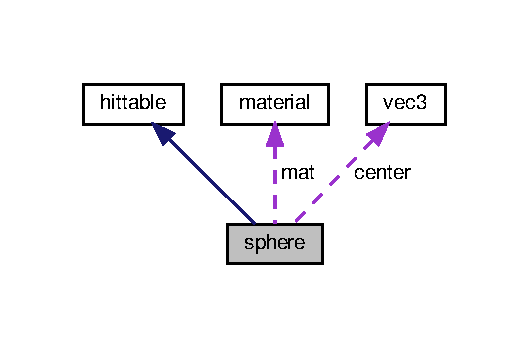
\includegraphics[width=254pt]{classsphere__coll__graph}
\end{center}
\end{figure}
\subsection*{Public Member Functions}
\begin{DoxyCompactItemize}
\item 
\mbox{\Hypertarget{classsphere_ab3f00cd2dc70110d320ffd73b165c0ba}\label{classsphere_ab3f00cd2dc70110d320ffd73b165c0ba}} 
{\bfseries sphere} (const \hyperlink{classvec3}{vec3} \&a, float b, \hyperlink{classmaterial}{material} $\ast$m)
\item 
\mbox{\Hypertarget{classsphere_a49d4617e15918e1dcaaf5156bb9b4252}\label{classsphere_a49d4617e15918e1dcaaf5156bb9b4252}} 
bool {\bfseries hit} (const \hyperlink{classray}{ray} \&r, float min, float max, \hyperlink{structhit__record}{hit\+\_\+record} \&rec) const
\end{DoxyCompactItemize}
\subsection*{Public Attributes}
\begin{DoxyCompactItemize}
\item 
\mbox{\Hypertarget{classsphere_a627be5e72c760037f7e976a00e14192c}\label{classsphere_a627be5e72c760037f7e976a00e14192c}} 
\hyperlink{classvec3}{vec3} {\bfseries center}
\item 
\mbox{\Hypertarget{classsphere_a9bad2d7ecf6f75cc998b893248fff8a2}\label{classsphere_a9bad2d7ecf6f75cc998b893248fff8a2}} 
float {\bfseries radius}
\item 
\mbox{\Hypertarget{classsphere_a206945004e5f943cdf78aa0f157c3c62}\label{classsphere_a206945004e5f943cdf78aa0f157c3c62}} 
\hyperlink{classmaterial}{material} $\ast$ {\bfseries mat}
\end{DoxyCompactItemize}


The documentation for this class was generated from the following file\+:\begin{DoxyCompactItemize}
\item 
sphere.\+h\end{DoxyCompactItemize}

\hypertarget{classvec3}{}\section{vec3 Class Reference}
\label{classvec3}\index{vec3@{vec3}}
\subsection*{Public Member Functions}
\begin{DoxyCompactItemize}
\item 
\mbox{\Hypertarget{classvec3_a4acbd353a5e121d018048b5f7391e841}\label{classvec3_a4acbd353a5e121d018048b5f7391e841}} 
\+\_\+\+\_\+host\+\_\+\+\_\+ \+\_\+\+\_\+device\+\_\+\+\_\+ {\bfseries vec3} (float a, float b, float c)
\item 
\mbox{\Hypertarget{classvec3_a4dc60158c63781877fb71ebff7c00303}\label{classvec3_a4dc60158c63781877fb71ebff7c00303}} 
\+\_\+\+\_\+host\+\_\+\+\_\+ \+\_\+\+\_\+device\+\_\+\+\_\+ \hyperlink{classvec3}{vec3} {\bfseries operator+} (const \hyperlink{classvec3}{vec3} \&v) const
\item 
\mbox{\Hypertarget{classvec3_ad283381c62ed9f6b78b50bf7a52c4516}\label{classvec3_ad283381c62ed9f6b78b50bf7a52c4516}} 
\+\_\+\+\_\+host\+\_\+\+\_\+ \+\_\+\+\_\+device\+\_\+\+\_\+ \hyperlink{classvec3}{vec3} {\bfseries operator-\/} (const \hyperlink{classvec3}{vec3} \&v) const
\item 
\mbox{\Hypertarget{classvec3_ae7e6adfaa2700354c81247bcd7e24841}\label{classvec3_ae7e6adfaa2700354c81247bcd7e24841}} 
\+\_\+\+\_\+host\+\_\+\+\_\+ \+\_\+\+\_\+device\+\_\+\+\_\+ \hyperlink{classvec3}{vec3} {\bfseries operator$\ast$} (const float \&s) const
\item 
\mbox{\Hypertarget{classvec3_ad700a89b0950d55f14edb06e828bcd58}\label{classvec3_ad700a89b0950d55f14edb06e828bcd58}} 
\+\_\+\+\_\+host\+\_\+\+\_\+ \+\_\+\+\_\+device\+\_\+\+\_\+ \hyperlink{classvec3}{vec3} {\bfseries operator$\ast$} (const \hyperlink{classvec3}{vec3} \&v) const
\item 
\mbox{\Hypertarget{classvec3_a8d988c6e85fcb6490c62c9dddcc089d6}\label{classvec3_a8d988c6e85fcb6490c62c9dddcc089d6}} 
\+\_\+\+\_\+host\+\_\+\+\_\+ \+\_\+\+\_\+device\+\_\+\+\_\+ \hyperlink{classvec3}{vec3} {\bfseries operator/} (const float \&s) const
\item 
\mbox{\Hypertarget{classvec3_a4d1a7c3c089c142283f8bba5b624188c}\label{classvec3_a4d1a7c3c089c142283f8bba5b624188c}} 
\+\_\+\+\_\+host\+\_\+\+\_\+ \+\_\+\+\_\+device\+\_\+\+\_\+ \hyperlink{classvec3}{vec3} {\bfseries operator/} (const \hyperlink{classvec3}{vec3} \&v) const
\item 
\mbox{\Hypertarget{classvec3_a71e4e115b861cee4f7054685fb8ae150}\label{classvec3_a71e4e115b861cee4f7054685fb8ae150}} 
\+\_\+\+\_\+host\+\_\+\+\_\+ \+\_\+\+\_\+device\+\_\+\+\_\+ \hyperlink{classvec3}{vec3} {\bfseries operator-\/} () const
\item 
\mbox{\Hypertarget{classvec3_ac338a08d2a16be3f1ca838b91e041263}\label{classvec3_ac338a08d2a16be3f1ca838b91e041263}} 
\+\_\+\+\_\+host\+\_\+\+\_\+ \+\_\+\+\_\+device\+\_\+\+\_\+ float {\bfseries dot} (const \hyperlink{classvec3}{vec3} \&v) const
\item 
\mbox{\Hypertarget{classvec3_a4d4fd63e75dfa34a32d2b859253756fc}\label{classvec3_a4d4fd63e75dfa34a32d2b859253756fc}} 
\+\_\+\+\_\+host\+\_\+\+\_\+ \+\_\+\+\_\+device\+\_\+\+\_\+ \hyperlink{classvec3}{vec3} {\bfseries cross} (const \hyperlink{classvec3}{vec3} \&v) const
\item 
\mbox{\Hypertarget{classvec3_a2c7fd1266bcedd021b2ae67ef74a60a9}\label{classvec3_a2c7fd1266bcedd021b2ae67ef74a60a9}} 
\+\_\+\+\_\+host\+\_\+\+\_\+ \+\_\+\+\_\+device\+\_\+\+\_\+ float {\bfseries magnitude} () const
\item 
\mbox{\Hypertarget{classvec3_a729bc59c5163d561f17ecc9fe6ec0394}\label{classvec3_a729bc59c5163d561f17ecc9fe6ec0394}} 
\+\_\+\+\_\+host\+\_\+\+\_\+ \+\_\+\+\_\+device\+\_\+\+\_\+ \hyperlink{classvec3}{vec3} {\bfseries normalize} () const
\end{DoxyCompactItemize}
\subsection*{Public Attributes}
\begin{DoxyCompactItemize}
\item 
\mbox{\Hypertarget{classvec3_a4ee2cfd5c2698031a47ab7f898d8d47b}\label{classvec3_a4ee2cfd5c2698031a47ab7f898d8d47b}} 
float {\bfseries x}
\item 
\mbox{\Hypertarget{classvec3_a891379795a14c80936cde4170239a138}\label{classvec3_a891379795a14c80936cde4170239a138}} 
float {\bfseries y}
\item 
\mbox{\Hypertarget{classvec3_aa76213efcc5d656cc14b71db80a92162}\label{classvec3_aa76213efcc5d656cc14b71db80a92162}} 
float {\bfseries z}
\end{DoxyCompactItemize}


The documentation for this class was generated from the following file\+:\begin{DoxyCompactItemize}
\item 
vec3.\+h\end{DoxyCompactItemize}

%--- End generated contents ---

% Index
\backmatter
\newpage
\phantomsection
\clearemptydoublepage
\addcontentsline{toc}{chapter}{Index}
\printindex

\end{document}
